%%%%%%%%%%%%%%%%%%%%%%%%%%%%%%%%%%%%%%%%%%%%%%%%%%%%%%%%%%%%%%%%%%
%
% Analysis of Algorithms
%
% Homework Assignment #6
%
%%%%%%%%%%%%%%%%%%%%%%%%%%%%%%%%%%%%%%%%%%%%%%%%%%%%%%%%%%%%%%%%%%
%%%%%%%%%%%%%%%%%%%%%%%%%%%%%%%%%%%%%%%%%%%%%%%%%%%%%%%%%%%%%%%%%%
%
% Score Card and Answer Sheets
%
%%%%%%%%%%%%%%%%%%%%%%%%%%%%%%%%%%%%%%%%%%%%%%%%%%%%%%%%%%%%%%%%%%
\documentclass[addpoints,11pt]{exam}
\usepackage{amsmath}
\usepackage{amstext}
\usepackage{clrscode3e}
\usepackage{enumitem}
\usepackage{fullpage}
\usepackage{xcolor}
\usepackage{graphicx}
\usepackage{amsmath}




%%%%%%%%%%%%%%%%%%%%%%%%%%%%%%%%%%%%%%%%%%%%%%%%%%%%%%%%%%%%%%%%%%
%
% Begin Document
%
%%%%%%%%%%%%%%%%%%%%%%%%%%%%%%%%%%%%%%%%%%%%%%%%%%%%%%%%%%%%%%%%%%
\begin{document}
\pagestyle{empty}


\noindent{\large\bfseries Name: Alfredo Perez}\\
\noindent{\large\bfseries COSC 40403 - Analysis of Algorithms: Homework 6}\\
\noindent{\large\bfseries Due: 23:30 on October 21}


%%%%%%%%%%%%%%%%%%%%%%%%%%%%%%%%%%%%%%%%%%%%%%%%%%%%%%%%%%%%%%%%%%
%
% Score Card and Answer Sheets
%
% Comment out one-or-the-other to show or not-show the answers.
%
%%%%%%%%%%%%%%%%%%%%%%%%%%%%%%%%%%%%%%%%%%%%%%%%%%%%%%%%%%%%%%%%%%
%\SolutionEmphasis{\color{violet}}

\renewcommand{\solutiontitle}{\noindent\textbf{Answer:}\par\noindent}

\printanswers
%%\noprintanswers



%%%%%%%%%%%%%%%%%%%%%%%%%%%%%%%%%%%%%%%%%%%%%%%%%%%%%%%%%%%%%%%%%%
% Begin Questions
%%%%%%%%%%%%%%%%%%%%%%%%%%%%%%%%%%%%%%%%%%%%%%%%%%%%%%%%%%%%%%%%%%
\begin{questions}


%%%%%%%%%%%%%%%%%%%%%%%%%%%%%%%%%%%%%%%%%%%%%%%%%%%%%%%%%%%%%%%%%%
% Question
%%%%%%%%%%%%%%%%%%%%%%%%%%%%%%%%%%%%%%%%%%%%%%%%%%%%%%%%%%%%%%%%%%
\question(\totalpoints \text{ points total})
Use the master method to give tight asymptotic bounds for the following recurrences.  Show your work to receive partial credit.
\begin{parts}
	\part [3] $T(n) = 2T(n/4) + 1$.
	\part [3] $T(n) = 2T(n/4) + \sqrt{n}$.
	\part [3] $T(n) = 2T(n/4) + n$.
	\part [3] $T(n) = 2T(n/4) + n^2$.
\end{parts}

\begin{solutionorbox}
Using the Master Method: \newline
a)\newline
 Compare $f(n)$ with $\log_{a}b $ where a = 2, b = 4, $f(n)$ = 1. \newline
$n^{\log_{a}b}$ = $n^{\log_{2}4} = \sqrt{n}$ $>$ $f(n)$ = 1 \newline
By knowing this we can deduce we have a time complexity of $\Theta(\sqrt{n})$\newline
b) \newline
Let a = 2, b = 4 \newline
$\log_{a}b $ = $\log_{2}4 $ = $n^2$ = $f(n)$ = $n^2$
The time complexity for this recurrence is $\Theta(f(n))\log_{n}$ = $\Theta(\sqrt{n}\log_{n})$ \newline
c) \newline
Let a = 2, b = 4 \newline
$\log_{a}b $ = $\log_{2}4 $ = $\sqrt{n}$ $<$ $f(n)$ = $n$
Thus, the time complexity is $\Theta(f(n)) = \Theta(n)$ \newline
d) \newline
Let a = 2, b = 4 \newline
$\log_{a}b $ = $\log_{2}4 $ = $\sqrt{n}$ $<$ $f(n)$ = $n^2$. \newline
Thus the time compelxity is of $\Theta(f(n)) = \Theta(n^2)$
\end{solutionorbox}

\ifprintanswers
\newpage
\else
\bigskip
\fi


%%%%%%%%%%%%%%%%%%%%%%%%%%%%%%%%%%%%%%%%%%%%%%%%%%%%%%%%%%%%%%%%%%%
%% Question
%%%%%%%%%%%%%%%%%%%%%%%%%%%%%%%%%%%%%%%%%%%%%%%%%%%%%%%%%%%%%%%%%%%
\question[8] Use Strassen's algorithm to compute the matrix product
$\begin{pmatrix}
	2 & 3\\
	5 & 7
\end{pmatrix}
$
$\begin{pmatrix}
	11 & 13\\
	17 & 19
\end{pmatrix}
$.  Show your work to receive partial credit.
\begin{solutionorbox}
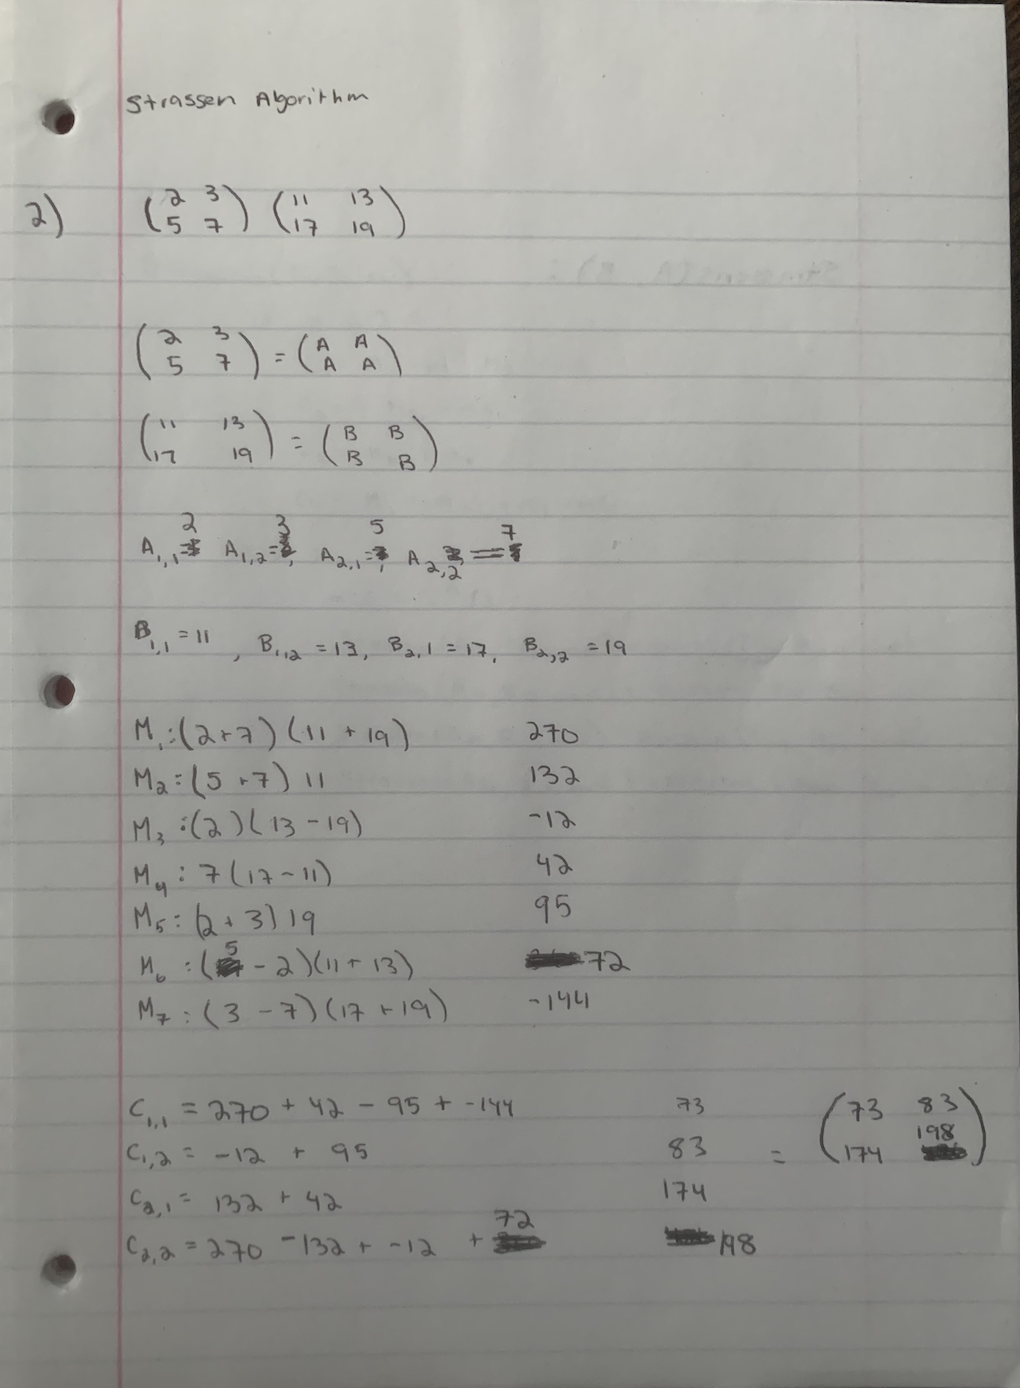
\includegraphics[width=5in]{no2}
\end{solutionorbox}

\ifprintanswers
\newpage
\else
\bigskip
\fi


%%%%%%%%%%%%%%%%%%%%%%%%%%%%%%%%%%%%%%%%%%%%%%%%%%%%%%%%%%%%%%%%%%%
%% Question
%%%%%%%%%%%%%%%%%%%%%%%%%%%%%%%%%%%%%%%%%%%%%%%%%%%%%%%%%%%%%%%%%%%
\question[10] Write pseudocode for Strassen's algorithm.  Do not write your algorithm in Python (or any other programming language).
\begin{solutionorbox}
	
	     Let A = $
	     \begin{bmatrix} 
	     	A^{11} & A^{12} \\
	     	A^{21} & A^{22}\\
	     \end{bmatrix}
	     $ and B = $
	     \begin{bmatrix} 
	     	B^{11} & B^{12}  \\
	     	B^{21} & B^{22} \\
	     \end{bmatrix}
	     $ \newline
	     Strassen(A,B): \newline
	     If n = 1 Return A x B \newline
	          Else: \newline
	     
	    $ M1 = Strassen(A^{11}, B^{12} - B^{22})$ \newline
	     $M2 = Strassen(A^{11} + A^{12}, B^{22})$\newline
	    $ M3 = Strassen(A^{21} + A^{22}, B^{11})$\newline
	     $M4 = Strassen(A^{22}, B^{21} - B^{11})$\newline
	    $ M5 = Strassen(A^{11} + A^{22}, B^{11} + B^{22})$\newline
	    $ M6 = Strassen(A^12 - A^{22}, B^{21} + B^{22})$\newline
	    $ M7 = Strassen(A^{11} - A^{21}, B^{11} + B^{12})$\newline
	    
	    $C^{11} = M_5 + M_4 - P_2 + P_6$ \newline
	    $C^{12} = M_1 + P_2$\newline
	    $C^{21} = M_3 + M_4$\newline
	    $C^{22} =M_1 + M_5 - M_3 - M_7 $	\newline
	    Return C     
\end{solutionorbox}

\ifprintanswers
\newpage
\else
\bigskip
\fi


%%%%%%%%%%%%%%%%%%%%%%%%%%%%%%%%%%%%%%%%%%%%%%%%%%%%%%%%%%%%%%%%%%%
%% Question
%%%%%%%%%%%%%%%%%%%%%%%%%%%%%%%%%%%%%%%%%%%%%%%%%%%%%%%%%%%%%%%%%%%
\question (\totalpoints \text{ points total}) 
The version of \proc{Partition} given in lecture is not the original partitioning algorithm.  Here is the original partition algorithm, which is due to C. A. R. Hoare in 1962.
\begin{codebox} \Procname{$\proc{Hoare-Partition}(A, p, r)$}
	\li $x = A[p]$
	\li $i = p - 1$
	\li $j = r + 1$
	\li \While \const{True} \Do
	\li     \Repeat
	\li         $j = j - 1$
	\li     \Until $A[j] \le x$
	\li     \Repeat
	\li         $i = i + 1$
	\li     \Until $A[i] \ge x$
	\li     \If $i < j$ \Then
	\li         $exchange A[i] with A[j]$
	\li     \Else
	\li         \Return $j$
			\End
		\End
\end{codebox}
Answer the following questions.  Show your work to receive partial credit.  Assuming $A[p \dots r]$ contains at least two elements, give a careful argument that the procedure \proc{Hoare-Partition} is correct and prove statements b, c, and d.

\begin{parts}
	\part [5] Demonstrate the operation of \proc{Hoare-Partition} on the array \\$A = \langle 21, 6, 2, 11, 4, 7, 8, 12, 5, 9, 19, 13 \rangle$, showing the values of the array and auxiliary values after each iteration of the while loop in lines 4-14.
	\part [5] The indices $i$ and $j$ are such that we never access an element of $A$ outside the subarray $A[p \dots r]$.
	\part [5] When \proc{Hoare-Partition} terminates, it returns a value j such that $p \le j < r$.
	\part [5] Every element $A[p \dots j]$ is less than or equal to every element of $A[j+1 \dots r]$ when \proc{Hoare-Partition} terminates.
	
\end{parts}

\begin{solutionorbox}
a) \newline

The first while loop (outer while) has swap when j = 12 and i =1
so we have A= [13, 6, 2, 11, 4, 7, 8, 12, 5, 9, 19, 21]. \newline
The second outer while loop ends when j = 11 and i = 12
and in this case no swap occurs because i $>$ j return j = 11
In the second outer while loop, we increase from 1 to 12 and A[12]= 21 $>=$ 21 is True, so it's done with this i inner loop and we start comparison between i and j. Since i $>$ j, it returns j = 11. \newline
b) \newline
This is correct, the indices i and j never have access to the element outside its subarray. 

As per partitioning we want every element to the left of pivot value to be less than or equal to the pivot and greater than on right side of pivot.

So we will move i marker untill we get element which is greater than or equal to pivot. We do the same with the j marker untill we find an element that is less than or equal to pivot.

When i $<$ j we swap the elements since both the elements are in wrong part of array. 

Now if i is not less than j,that means now there is no element in between to swap so we return j position.

So now the array after partitioned lower half is from (start to j) while the upper half is from (j+1 to end).

Therefore the two indeces remain partitioned and separate from each other.
\newline
c) \newline
This is true because the value of j will always be between the low(p) and high(r) values of the array. J is greater than or equal to p since it might be the initial value in the array. \newline
d) \newline
This is true since the elements in A[p$\dots$j] will be the elements which have been partitioned in the lower half. The elements of A[j+1 ... r] are in the right side of the pivot. Thus, the values of A[p...j] will always be less than or equal to the elements of A[j+1 ... r].


\end{solutionorbox}


%%%%%%%%%%%%%%%%%%%%%%%%%%%%%%%%%%%%%%%%%%%%%%%%%%%%%%%%%%%%%%%%%%
%%%%%%%%%%%%%%%%%%%%%%%%%%%%%%%%%%%%%%%%%%%%%%%%%%%%%%%%%%%%%%%%%%
\end{questions}


%%%%%%%%%%%%%%%%%%%%%%%%%%%%%%%%%%%%%%%%%%%%%%%%%%%%%%%%%%%%%%%%%%
%%%%%%%%%%%%%%%%%%%%%%%%%%%%%%%%%%%%%%%%%%%%%%%%%%%%%%%%%%%%%%%%%%
\end{document}
